\documentclass{article}
\usepackage[UTF8]{ctex}


\usepackage[utf8]{inputenc} % allow utf-8 input
\usepackage[T1]{fontenc}    % use 8-bit T1 fonts
\usepackage{hyperref}       % hyperlinks
\usepackage{url}            % simple URL typesetting
\usepackage{booktabs}       % professional-quality tables
\usepackage{amsfonts}       % blackboard math symbols
\usepackage{nicefrac}       % compact symbols for 1/2, etc.
\usepackage{microtype}      % microtypography
\usepackage{lipsum}
\usepackage{amsmath}
\usepackage{amssymb}
\graphicspath{{/home/yan/Documents/Texstudion_project/figure/}}

\title{deep learning 算法}


\author{
  HengGeZhiZou\\
  \texttt{1018676477@qq.com} \\
  %% \AND
  %% Coauthor \\
  %% Affiliation \\
  %% Address \\
  %% \texttt{email} \\
  %% \And
  %% Coauthor \\
  %% Affiliation \\
  %% Address \\
  %% \texttt{email} \\
  %% \And
  %% Coauthor \\
  %% Affiliation \\
  %% Address \\
  %% \texttt{email} \\
}

\begin{document}
\maketitle

\begin{abstract}
本文总结目前学习的深度学习算法,主要用于text classification方向
\end{abstract}


\section{Introduction}

文本分类作为nlp中基础部分,也是许多算法的出发点,在一段时间的学习后,我们总结目前的一些基本算法。

\section{文本分类算法}
按顺序总结cnn,fasttext,rnn,rcnn,seq2seq with attention,Hierarchical Attention Network,transform,ELMO,
BERT等算法。


\subsection{CNN: 卷积神经网络 }
利用CNN作文本分类的想法来自于Yoon Kim[1]。在他的文章中,将卷积运算对文本的信息进行提取,取得了非常不错的效果。在文本分类中,上下文词汇一般具有关系,我们在分类时注意上下文的关系往往能够提升算法的效果。

一般cnn分成输入层,卷积层,池化层,全连接层的多层结构。

输入层作为cnn的第一层,将句子中的词嵌入到向量空间中。一般我们用input=[batch size ,sequence length]作为整个cnn的输入,其中batch size代表我们输入训练集句子的数量。sequence length代表这些句子的最大长度。输入构成一个2维的tensor,在axis=0方向上是batch size,在axis=1方向上是sequence length 个词,即为每一句话的词。通常我们将每一个字用数字表示(建立词汇表)。对于第一步将句子嵌入到向量空间,我们有两种做法。第一种是我们初始化一个大小为[vocabulary size ,word embedding size]的矩阵,一般我们用随机生成一个均匀分布的映射矩阵W。第二种我们使用已经预训练好的嵌入矩阵,他的大小和第一种方式相同。从实验的结果来看,第二种方法的损失函数收敛速度更快,但是对最后的结果影响不大(两个词嵌入矩阵会在训练过程中更新)。我们通过查找的方法,将input中的词在词汇表W找到对应的词向量
,得到一个大小为[batch size,sequence length,word embedding size]的输入tensor叫做embeddedchar。

卷积层作为卷积神经网络的核心,我们使用不同的卷积核对原始的embeddedhar进行卷积运算,我们一般选择不同filter window size ,在图中选择[2,3,4]。在文本分类任务中,卷积核的宽度和词向量的维度相等。于是我们的卷积核大小为[filter window size,word embedding size,channel,num filters]其中channel为卷积的通道数,一般embeddedhar的通道数为1,num filters 为相同卷积窗口大小卷积核的数量。使用不同大小的卷积窗口计算的得到的feature map长度也h不同(sequence length - filter window size + 1)。计算结果的大小为[batch,h,1,num filters],同时我们需要对feature map 进行一个relu 的activation function。

池化层对feature map 中的结果进行计算,取出每一个feature map中的最大值,代表当前卷积核运算的结果,将相同卷积窗口大小的结果进行concat,然后将所有的不同卷积窗口的计算机结果再次进行concat。得到最终大小为[batch,num filter size * 选择不同窗口的卷积核的数量]。

全连接层对池化层的结果进行计算,我们初始化一个大小为[num filter size * 选择不同窗口的卷积核的数量, num classes]的权值矩阵,同时使用截断正太分布。通过全连接层后softmax得到最终的结果。[batch size,num classes]。最后我们通过损失函数来梯度下降更新全部参数。

有一点需要注意的是我们在文本分析中,没有图像RGB的多通道,但是我们可以在词嵌入时使用不同的词汇表作为多个通道(word2vec,glove等等)。


\begin{figure}
  \centering
  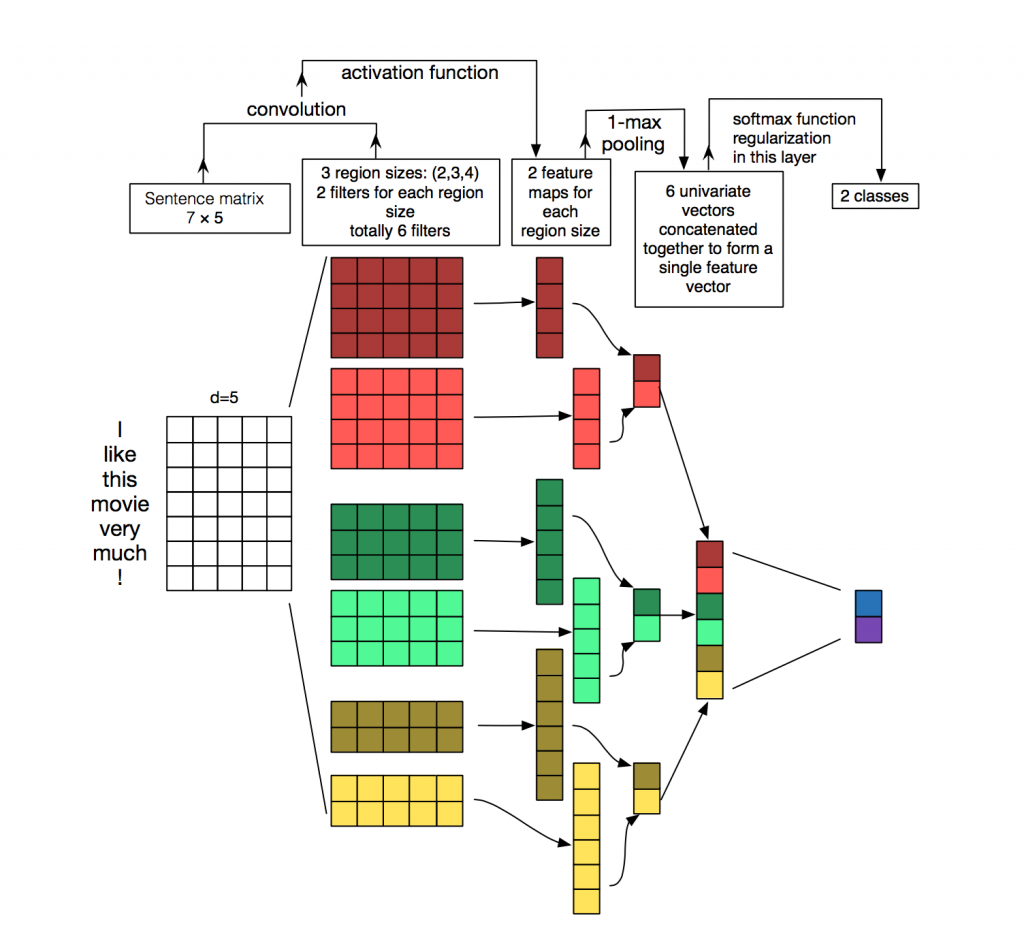
\includegraphics[width=.8\textwidth]{cnn.png} %1.png是图片文件的相对路径
  \caption{cnn 文本分类结构}
  \label{fig:fig1}
\end{figure}



\subsection{FASTTEXT}
 
 fasttext的网络结构相对简单,输入一个词的序列或者是一句话,最后的得到这个词序列的类别标签。
 
 
 在fasttext中,我们不仅使用每一个词的嵌入向量,为了不漏掉一些词意的微小变化,例如un,dis这些词缀,我们同时可以使用字符级的n-gram来增加一些的新的特征提高整个模型的准确率。训练的输入[batch size,sequence length ],通过输入层进行词嵌入后,得到[batch size,sequence length ,embedding size],在hidden layer 我们将上一层的输出向量进行平均,得到一个大小为[batch size,embedding size]的tensor,其中每一个tensor都代表开始输入的词序列。然后通过一个全连接层[embedding size,num classes ]得到类别结果。

为了改善运算的速度,模型使用了层级softmax,和传统的softmax会计算所有的元素值不同,层级softmax在生成词向量中,由于词汇表具有大量单词,而通过[embedding size, vocabulary size]的全连接层和softmax后需要耗费大量的计算资源,于是我们需要层次softmax。而在普通文本分类任务中,类别一般较少,没有必要使用层次softmax。
\begin{figure}
  \centering
  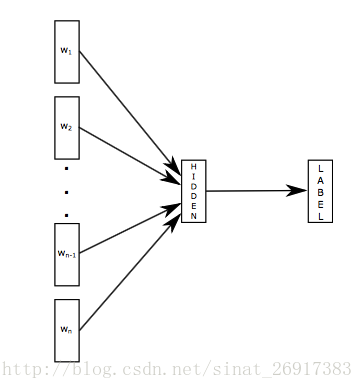
\includegraphics[width=.8\textwidth]{fasttext.png} %1.png是图片文件的相对路径
  \caption{fasttext结构}
  \label{fig:fig1}
\end{figure}




\subsection{RNN}

rnn循环神经网络是深度学习中必不可少的一种算法。从人类的语言角度出发,上下文之间存在着强烈的关联,往往每一个单词都不会单独只有本身的意义。和上下文之间的联系使得rnn的结构和句子序列结构十分契合。我们首先看看一般基本的rnn结构:

\begin{figure}
  \centering
  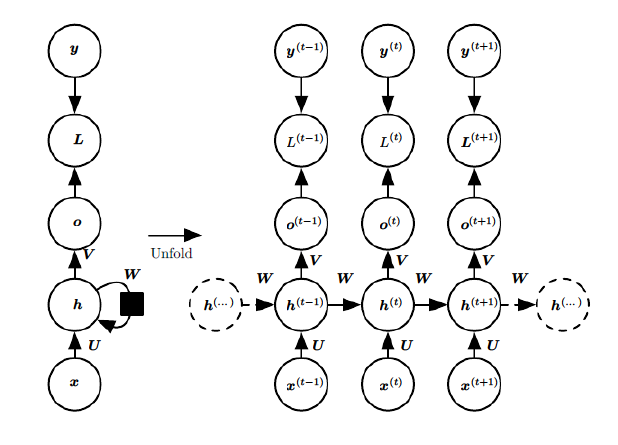
\includegraphics[width=.8\textwidth]{rnn.png} %1.png是图片文件的相对路径
  \caption{rnn文本分类结构}
  \label{fig:fig1}
\end{figure}


其中x为序列输入的词,一般输入为一个完整的句子。输入大小为[batch size,sequence length],首先经过一个词嵌入层,将所有的句子中的词映射到线性空间,生成的输入为[batch ,sequence length ,  embedding size]。让后将句子序列输入到rnn中。其中每一层的rnn都共享权重参数,即U,W,V全部相同,每一个时刻hidden state 的输入为当前词的输入和上一个hidden state 的输出,在cell中经过一个activation function为当前cell的输出,当前的输出一部分作为当前时间步的输入o。另一部分传输到下一个神经单元。对o使用激活函数后就为最终的输出。大小为[batch ,sequence length, hidden state size] ,在sequence 方向上依次为每一个词输入的输出。通常我们在进行文本分类时一般选取最后一个序列的输出作为最后的输出。虽然这样有一定的局限,比如过长的句子会使得rnn遗忘掉开始的内容。选择最后一个输出则大小为[batch size,1,hidden state size],在通过一个权值为[hidden state size,num classes] 的全连接层,我们得到最后的分类结果。我们在进行梯度下降更新参数的时候又遇到了另外一个关键的问题。

首先我们更新最近的参数V
\begin{figure}
  \centering
  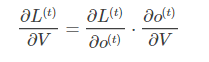
\includegraphics[width=.8\textwidth]{v.png} %1.png是图片文件的相对路径
  \caption{v}
  \label{fig:fig1}
\end{figure}

v的参数更新比较容易,我们只需要关注目前的输出,将损失函数对v求导。由于时序列化的结构,我们会得到多个单元的不同输出,于是我们求解每一个时刻输出后进行损失的求和:
\begin{figure}
  \centering
  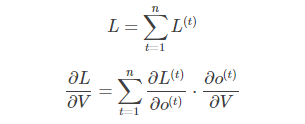
\includegraphics[width=.8\textwidth]{derivative.png} %1.png是图片文件的相对路径
  \caption{derivative}
  \label{fig:fig1}
\end{figure}


然而在对于W和U的求导过程中,由于显示序列化的数据,会链式对一个参数求导:
\begin{figure}
  \centering
  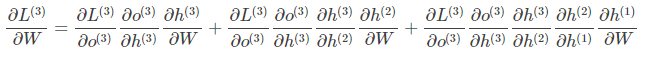
\includegraphics[width=.8\textwidth]{chain rule.png} %1.png是图片文件的相对路径
  \caption{chain rule w}
  \label{fig:fig1}
\end{figure}

同时对U的求导过程和W相同,我们得到一个通式:

\begin{figure}
  \centering
  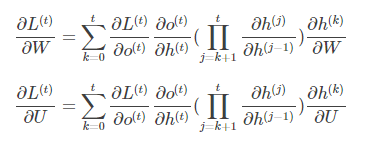
\includegraphics[width=.8\textwidth]{rule.png} %1.png是图片文件的相对路径
  \caption{rule}
  \label{fig:fig1}
\end{figure}


其中我们把中间的一项导数求得结果为:

\begin{figure}
  \centering
  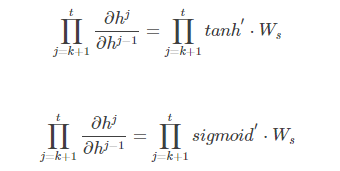
\includegraphics[width=.8\textwidth]{result.png} %1.png是图片文件的相对路径
  \caption{result}
  \label{fig:fig1}
\end{figure}

其中我们使用了不同的激活函数,tanh和sigmoid两种不同的激活函数。然而在对这两种激活函数的求导过程中我们发现了问题,

\begin{figure}
  \centering
  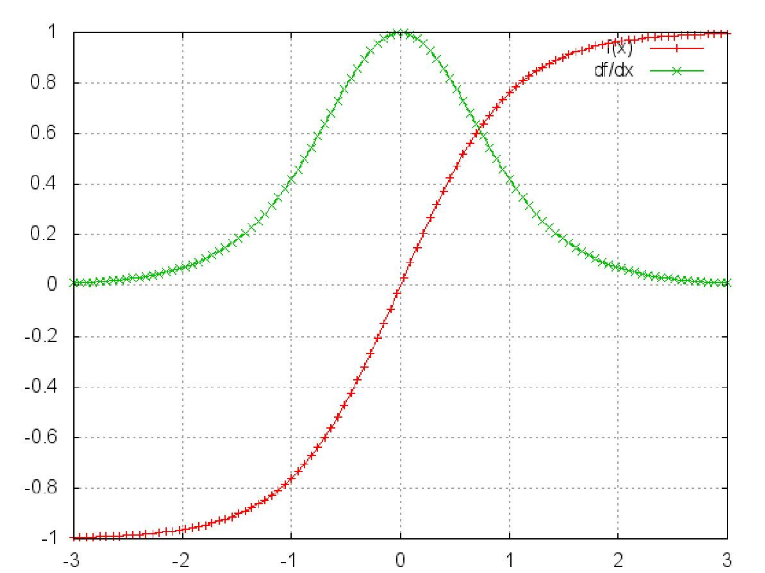
\includegraphics[width=.8\textwidth]{tanh.png} %1.png是图片文件的相对路径
  \caption{result}
  \label{fig:fig1}
\end{figure}
\begin{figure}
  \centering
  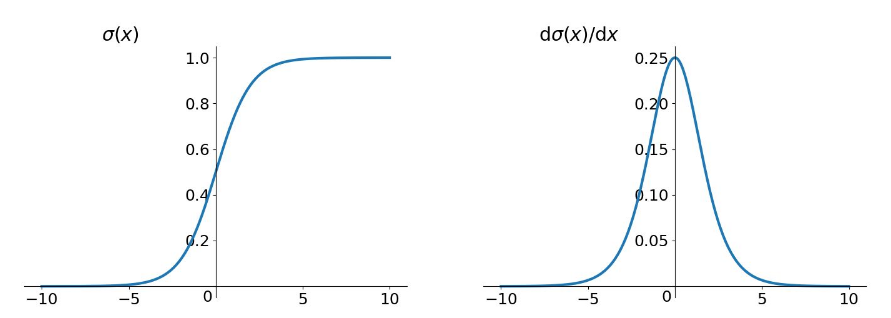
\includegraphics[width=.8\textwidth]{sigmoid.png} %1.png是图片文件的相对路径
  \caption{result}
  \label{fig:fig1}
\end{figure}

两种激活函数的导数大小都在0和1之间,当rnn中hidden state 的层较多时,在不断累乘的过程中,梯度可能会无限接近0,或者很大,导致我们的无法正常更新参数。也就是‘梯度消失’和‘梯度爆炸’。为了解决梯度更新的问题,以及上文中我们说到的由于长时间的传导,导致最后对前文的内容已经遗忘过多。


\subsection{LSTM}

LSTM将rnn中的普通cell更换为另外一种形式:

\begin{figure}
  \centering
  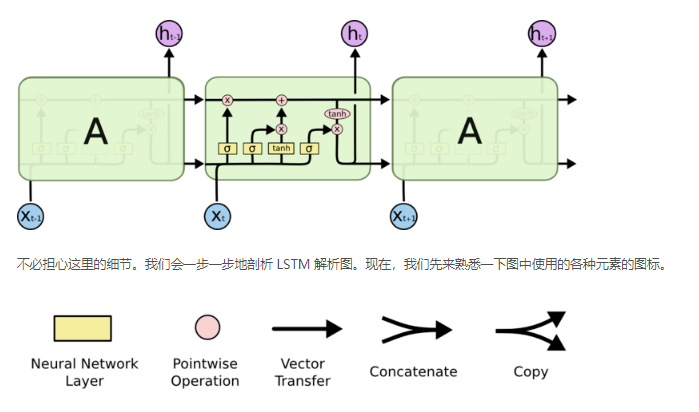
\includegraphics[width=.8\textwidth]{lstm.png} %1.png是图片文件的相对路径
  \caption{lstm}
  \label{fig:fig1}
\end{figure}

在LSTM中,为了对信息进行选择,共有三个门结构。分别为forget gate,input gate,output gate。

在forget gate中,我们将上一个cell的输出和当前时间步的输入进行结合,然后通过一个sigmoid激活函数得到ft(0,1),决定将上一个cell传达的信息保留多少,为0时全部丢弃,为1时全部保留。然后将ft和上一个细胞的输出相乘,得到我们需要保留的信息ft*ct-1。

在input gate中,第一步我们同样得到一个it,决定我们会更新当前的哪些值,同时将上一个cell的hidden state和当前时间步的输入结合通过一个tanh激活函数得到ct,然后将it和ct相乘,决定将要保留多少重要的信息。然后我们将当前的结果和it*ct-1相加得到ct。这是作为时间步向下一个cell的输出。并且如果在forget gate中的值接近0,那门可能drop掉许多信息。

在output gate中,决定当前cell的输出h,同样先经过一个forget gate,然后和ct相乘,得到输出ht,分别输出和传入下一个cell。

通过以上 的三个状态门,我们解决了信息传递丢失的问题,下面我们看看如何解决gradient vanish的问题。在对ct-1求导的过程中,后一项的数值大于0且为加法,我们可以只看主体部分,主体部分为一个值在0到1之间的数,所以避免了梯度消失。


\subsection{GRU}

作为rnn的另外一种变体结构,GRU具有两个门结构,更新门和重置门。

\begin{figure}
  \centering
  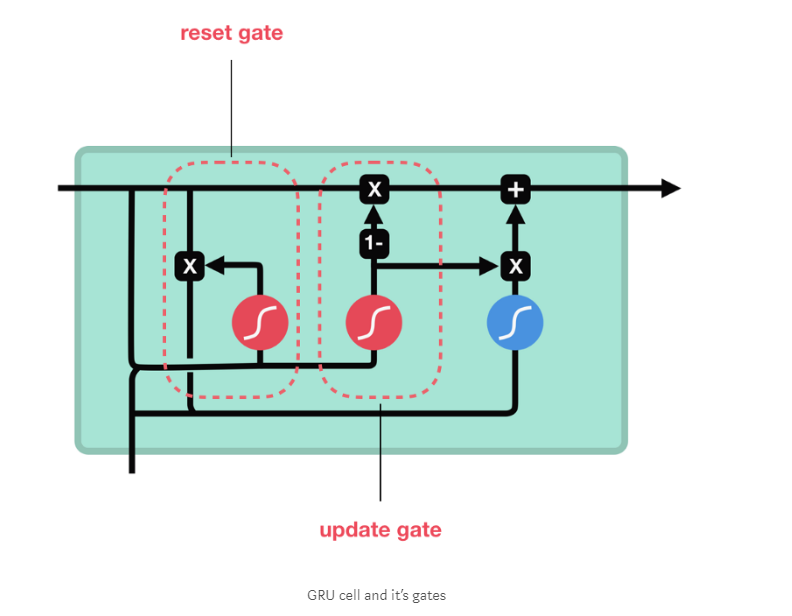
\includegraphics[width=.8\textwidth]{GRU.png} %1.png是图片文件的相对路径
  \caption{GRU}
  \label{fig:fig1}
\end{figure}


\subsection{Bi-rnn}
在 rnn中,往往只有前向序列的句子信息,也就是说一般当前词只包含了前方词语的信息。然而对于一些词来说,后面的部分也会对其产生一定的影响,于是使用双向的rnn能够获取到后方传递的信息。双向rnn的结构:

\begin{figure}
  \centering
  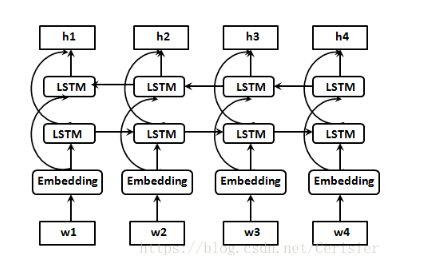
\includegraphics[width=.8\textwidth]{bi-rnn.png} %1.png是图片文件的相对路径
  \caption{GRU}
  \label{fig:fig1}
\end{figure}

同时双向rnn中的cell可以换成LSTM或者GRU。


\subsection{rcnn}

为了解决当前输入的词汇和上下文之间的联系问题,一种基于rnn和cnn的结构产生了。rcnn能够将一句话中上下文词意融合到每一个词中。使得每一个词都包含更多的信息。rcnn的结构为:

\begin{figure}
  \centering
  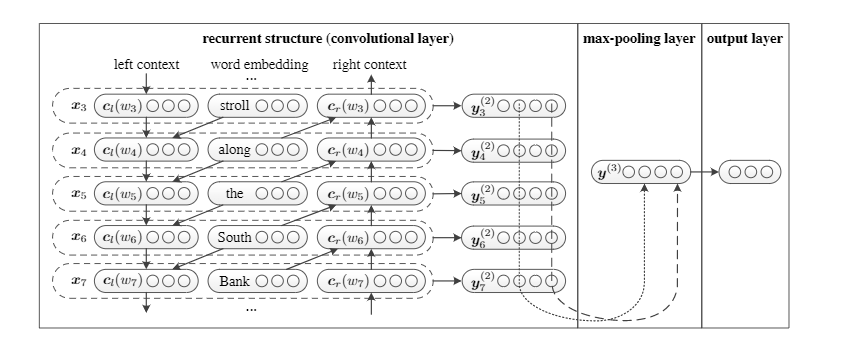
\includegraphics[width=.8\textwidth]{rcnn.png} %1.png是图片文件的相对路径
  \caption{rcnn}
  \label{fig:fig1}
\end{figure}

为了收集上下文对某一个词的影响,利用双向循环网络。在网络的第一层,正向输入句子序列,也就是每一个神经单元都可以获取当前输入以前的句子信息。输入同样为[batch size,embedding sequence length],首先将所有的输入嵌入到向量空间得到[batch size,sequence length,embedding size]的输入。然后我们对整个输入进行调整,将所有的句子按单词顺序划分,即每一句话的第一个词,第二个词....分别放在一组,得到一个长度为sequence length 的[batch size,embedding size ]大小的tensor。然后在一开始我们初始化一个随机词向量[batch size,embedding size] c left word ,作为第一个词的左边的词。同时我们初始化一个权值W left context作为在第一层循环神经网络之间传播的参数,它也可以看作我们初始化词左边的文章内容。然后将他们输入到一个神经单元,得到当前输入词左边的内容[batch size,embedding size]。相反,我们将输入反序输入,得到一个词汇右边的内容[batch size,embedding size]。然后我们将当前词左边的内容,当前词,当前词右边的内容进行结合。得到一个大小为[batch size,3*embedding size ]的tensor,其中每一个代表了输入词和他的上下文内容的信息。将tensor还原,得到一个[batch size,sequence length,3*embedding size ]的tensor,他保存着每一个句子中每一个融合了上下文信息的单词。以上是作为rcnn中的双向循环网络。然后将其通过一个最大池化层,将[batch size,sequence length ,3*embedding size]在axis=1的方向上求最大值,得到一个大小为[batch size ,1,3*embedding size]的tensor,他代表着一个句子的所有信息。通过全连接层后的得到我们最后的计算结果。

rcnn能够收集到上下文的信息对某个词的影响,同时他还融合了cnn中的最大池化层,作为句子信息的提炼。经过实验,效果良好



\subsection{seq2seq with attention}

作为在翻译领域提出的模型,seq2seq分为encoder和decoder两个部分。用一个循环神经网络将句子编码以后,通过另一个循环神经网络解码,这样可以翻译两种语言的不同长度句子。在seq2seq的基础上进一步加入了attention机制,使得整个文本中重要的部分得到提升,不重要的地方弱化。seq2seq with attention的具体结构为:

\begin{figure}
\centering
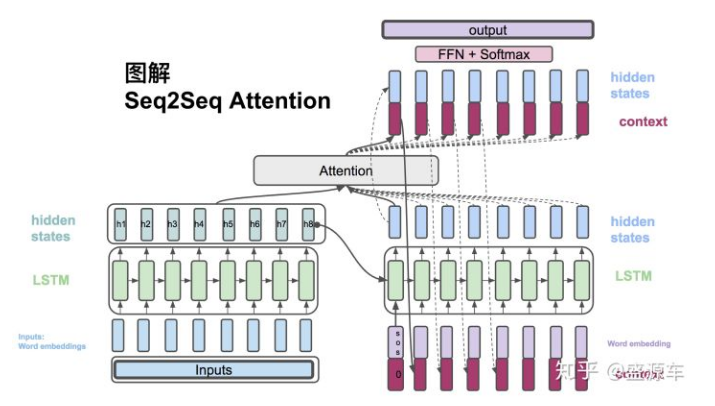
\includegraphics[width=.8\textwidth]{seq2seqattention.png}
\end{figure}


本来模型是作用在翻译领域,但是经过改造也可以用在多文本分类上。作为文本的输入,同样是[batch size,sequence length ]代表batch size个长度为sequence length的句子输入,然后将输入嵌入到词向量空间[batch size, sequence length ,embedding size].

encoder部分:使用一个双向GRU来作为句子的编码层:我们会得到两个输出。每一个GRU的双向单元会输入一个hidden state,大小为[batch size,hidden size]ht,同时将上一个GRU单元输出ht和当前的词作为下一个GRU单元的输入,得到GRU单元的输出。由于时双向GRU网络,每一层都会得到一个大小为[batch size,sequence  length,hidden size  ]的输出,将两层GRU的输出concat,得到一个大小为[batch size,sequence length,hidden size *2]的tensor。将两层最后一次的输出进行结合,得到一个[batch size, hidden size *2]的encoder结果。

decoder部分:作为多分类任务,每一个句子都有多个属性标签。label为[batch size ,decoder length size ]。为了将label嵌入到向量空间,首先初始化一个[ num classes,embedding size *2]大小的标签tensor,其中每一个label都初始化一个tensor。在训练阶段,将我们的结果先嵌入到向量空间中,得到一个大小为[batch size,decoder length size,embedding size *2]的tensor,代表每一个类别的tensor。也是作为解码阶段的输入。
同样,我们将类别tensor按顺序划分,即第一类,第二类...,得到一个长度为decoder length的[batch size,embedding size*2]的label。在解码部分我们同样使用一个双向的GRU解码网络,解码网络的输出为,上一个cell的输出,当前句子的类别标签,经过attention后的context。其中attention有多种方式:

\begin{figure}
\centering
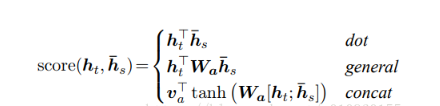
\includegraphics[width=.8\textwidth]{attention.png}
\end{figure}

我们选择第三种作为attention的方式。首先初始化一个大小为[hidden size ,hidden size]的权重tensor为Wa,将上一个cell的输出结果hs和Wa相乘,然后将在解码层的全部输出和Wa相乘,对两者相求和后通过激活函数tanh,然后和大小为[hidden size ,1]的Va相乘,从而得到一个attention的打分。attention的方式也就是上文中的concat。将计算得到的score和我们上面解码网络中的out进行multiply,对每一个hidden state的结果进行打分,然后求解在axis=1上的最大值,得到最后经过attention后的context。然后放入GRU计算单元中,得到最新的hidden state的输出。


解码完成后,我们通过一个全连接层得到最后计算结果。

\subsection{Hierarchical Attention Network}

多层注意力网络是做为文档分类的一种重要算法。他收集每一个句子的信息,然后将句子的信息汇集成文档的信息。从而对文档进行分类,他的模型结构为:

\begin{figure}
\centering
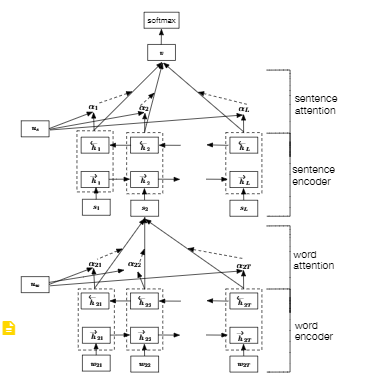
\includegraphics[]{hattention.png}
\end{figure}


作为文档,输入为[batch size, article length ,sentence length],其中article length 为每一篇文档的句子数量,sentence length为每一句话的长度。同样我们要将这些文章的词嵌入到向量空间,得到一个大小为[batch size,article length, sentence length ,word embedding size ]的输入tensor。我们对文章进行分割,得到一个长度为article length大小为[batch size,sentence length,word embedding size]的序列,其中每一组数据代表着每篇文章中的一句话。先对每一句话使用一个双层的LSTM或GRU进行信息选取,在LSTM的输出层后加入一个attention层,得到每一句话经过attention后的结果。然后在进行句子信息的提炼,得到最后的文章信息结果。





\begin{thebibliography}{1}

\bibitem{kour2014real}
George Kour and Raid Saabne.
\newblock Real-time segmentation of on-line handwritten arabic script.
\newblock In {\em Frontiers in Handwriting Recognition (ICFHR), 2014 14th
  International Conference on}, pages 417--422. IEEE, 2014.

\bibitem{kour2014fast}
George Kour and Raid Saabne.
\newblock Fast classification of handwritten on-line arabic characters.
\newblock In {\em Soft Computing and Pattern Recognition (SoCPaR), 2014 6th
  International Conference of}, pages 312--318. IEEE, 2014.

\bibitem{hadash2018estimate}
Guy Hadash, Einat Kermany, Boaz Carmeli, Ofer Lavi, George Kour, and Alon
  Jacovi.
\newblock Estimate and replace: A novel approach to integrating deep neural
  networks with existing applications.
\newblock {\em arXiv preprint arXiv:1804.09028}, 2018.

\end{thebibliography}

网络见图\ref{networkvgg}:

\begin{figure}[h]
	\centering
	\includegraphics[scale=0.3]{vgg16.pdf}
	\caption{网络图}\label{networkvgg}
\end{figure}


%$$	\sum_{l=1}^{L}{\sum_{j=1}^{c}({y^l_j}\times log({o^l_j})} + (1-{y^l_i}\times log(1-{o^l_j})) $$

损失函数:\begin{gather}
	LASS=\sum_{l=1}^{L}{\sum_{j=1}^{c}({y^l_j}\times log({o^l_j})} + (1-{y^l_i}\times log(1-{o^l_j}))
\end{gather}

\begin{gather}
\sum_{l=1}^{L}{\sum_{j=1}^{c}({y^l_j}\times log({o^l_j})} + (1-{y^l_i}\times log(1-{o^l_j}))
\end{gather}


\end{document}




